\section{Two separately registered local update realizations}
\label{sec:architectures}

Both candidates live on an oriented periodic cycle of $N$ cells with
directional labels $R$ and $L$.  Registered states occupy the global
one-excitation sector of dimension $2N$.  The direct registration declares an
explicit four-dimensional hard-core-qubit cell and full-space gates.  The
earlier product registration assigns local Hilbert dimension four and declares
ordinary transport SWAPs, but specifies its mass mixer only on the
one-excitation $R/L$ block.  Its vacuum and double-occupation phases are
therefore not frozen.  Both update laws are fully specified on the registered
one-excitation sector, but the comparison cannot use the product collision lift
to establish full-space update inequivalence.

\subsection{Ordered product walk}

The product candidate applies, from right to left,
\begin{equation}
  U_{\PW}[q]=S\,C_m[q]\,P_V[q],
  \label{eq:product-step}
\end{equation}
where
\begin{align}
  P_V[q]\lvert j,s\rangle
    &=e^{-\iu\Delta V_q(x_j)}\lvert j,s\rangle,\\
  C_m[q]
    &=e^{-\iu\Delta m_q\sigma_x},\\
  S\lvert j,R\rangle&=\lvert j+1,R\rangle,\qquad
  S\lvert j,L\rangle=\lvert j-1,L\rangle.
\end{align}
The transport $S$ is not counted as a free relabelling.  An on-site SWAP
followed by a directed edge SWAP realizes the two conditional shifts.  In the
frozen, unoptimized decomposition, a free macrostep has depth three and
gate-work $3N$; an active potential adds one leading phase layer and $N$ gates.
The free momentum block is
\begin{equation}
 U_{\PW}(k;m)=e^{-\iu\Delta k\sigma_z}e^{-\iu\Delta m\sigma_x}.
 \label{eq:product-block}
\end{equation}
Its leading global discrepancy is first order in $\Delta$, reflecting the
commutator of the ordered kinetic and mass factors
\citep{Arrighi2014DiracWalk}.

Because the product mass mixer lacks frozen $\lvert00\rangle$ and
$\lvert11\rangle$ actions, many full-space extensions share
Eq.~\eqref{eq:product-block}.  The natural hard-core extension
$\operatorname{diag}(1,e^{-\iu\Delta m\sigma_x},1)$ would carry the same
$+1$ double-occupation phase as the direct gates.  No product multiparticle or
collision-sector distinction is claimed.

\subsection{Direct symmetry-derived QCA}

For $q=k\Delta$, $\mu=m\Delta$, and $n=\sqrt{1-\mu^2}$, the established direct
one-excitation law has momentum block
\begin{equation}
 U_\mu(q)=
 \begin{pmatrix}
   ne^{-\iu q}&-\iu\mu\\
   -\iu\mu&ne^{\iu q}
 \end{pmatrix},
 \label{eq:direct-block}
\end{equation}
or real-space recurrence
\begin{equation}
 \begin{split}
 R'(x)&=nR(x-1)-\iu\mu L(x),\\
 L'(x)&=-\iu\mu R(x)+nL(x+1).
 \end{split}
 \label{eq:direct-recurrence}
\end{equation}
The law and its symmetry origin are prior art
\citep{Bisio2015QuantumFieldQCA,DAriano2014InformationPrinciples}.  What must be
declared for the present test is its finite full-space lift, circuit clock, and
collision boundary.

On edge subcells $(L_x,R_{x-1})$, in basis
$\lvert00\rangle,\lvert01\rangle,\lvert10\rangle,\lvert11\rangle$, define
\begin{equation}
 b_\mu=
 \begin{pmatrix}
 1&0&0&0\\
 0&-\iu\mu&n&0\\
 0&n&-\iu\mu&0\\
 0&0&0&1
 \end{pmatrix}.
 \label{eq:edge-gate}
\end{equation}
All disjoint edge gates form $B_\mu$; ordinary on-site SWAPs form $A$.  With
an optional leading number phase $P_V$, the physical macrostep is
\begin{equation}
  U_{\DQCA}[q]=A\,B_{\mu_q}\,P_V[q].
  \label{eq:direct-full-step}
\end{equation}
The one-excitation restriction of Eq.~\eqref{eq:direct-full-step} is exactly
Eq.~\eqref{eq:direct-recurrence}, coefficient by coefficient.  Each edge gate is
unitary because its one-excitation block is $nX-\iu\mu I$ and
$n^2+\mu^2=1$; the vacuum and double-occupation blocks are identities.  The
two partition layers are homogeneous and disjoint within a layer.  In its
frozen decomposition, one macrostep has radius one, free depth two, free
gate-work $2N$, and no ancilla.

This lift is an ordinary hard-core occupation-qubit QCA.  It fixes
$\lvert11\rangle$ with phase $+1$.  Canonical fermionic second quantization of
the same one-particle two-mode block would apply its determinant, $-1$, in the
double-occupation sector.  The two lifts agree on vacuum and one excitation
but need not agree on multiparticle scattering or spectrum
\citep{Farrelly2014CausalFermions,Mlodinow2020QFTQCA}.  The difference is an
explicit claim boundary, not a hidden implementation detail.

\subsection{Exact time-frame relation and different registered circuits}

The one-excitation blocks are algebraically close.  With
$K(q)=e^{-\iu q\sigma_z}$, the explicit half-step
$K(q)^{1/2}:=e^{-\iu q\sigma_z/2}$, and $\theta_\mu=\arcsin\mu$, the direct block obeys
\begin{equation}
 U_\mu(q)=K(q)^{1/2}e^{-\iu\theta_\mu\sigma_x}K(q)^{1/2}
 =K(q)^{-1/2}\!\left[K(q)e^{-\iu\theta_\mu\sigma_x}\right]K(q)^{1/2}.
 \label{eq:time-frame-relation}
\end{equation}
Discrete-time quantum walks admit unitarily related stroboscopic time frames,
conventionally represented by cyclic factor orderings $U'=FG$ and $U''=GF$
\citep{AsbothObuse2013TimeFrames}.  Equation~\eqref{eq:time-frame-relation}
is the model-specific instance here: the direct block is exactly a symmetric
split and is conjugate to a product-walk
block after the mass-angle remapping $\Delta m\mapsto\arcsin(m\Delta)$.  This
identity is a claim boundary, not a defect to conceal.  The conjugating factors
are chiral half-cell phases, not the integer-cell transport layers of the
registered product circuit.  The frozen specifications use different gate
partitions, intervention parameterizations, and protocol clocks.
The phrase \emph{two registered updates} therefore means two declared
one-excitation realizations under the fixed cell partition, encoding,
intervention map, and macrostep accounting.  It does not mean inequivalence
under arbitrary momentum-dependent frame changes or circuit resynthesis.

The resource difference is equally convention-bound.  In the product clock an
adjacent mass mixer and SWAP can be fused as
$X e^{-\iu\theta X}=\cos\theta\,X-\iu\sin\theta\,I$, the same
parameterized one-excitation form used by the direct edge scatter after the
time-frame change.  A library that treats arbitrary two-mode unitaries as
primitives can therefore compress
the product clock, while a SWAP-plus-rotation library would decompose the
direct scatter.  We report the sealed, nonminimal layer and gate counts because
they make the executed protocols auditable, not as compilation-invariant
complexity or a resource advantage.

On the principal small-step branch, the direct block's exact effective
generator is
\begin{equation}
 H_{\mathrm{eff}}(k,\Delta)
 =H_D(k)+\Delta^2K_2(k,m)+O(\Delta^4),
 \qquad H_D(k)=k\sigma_z+m\sigma_x,
 \label{eq:direct-effective}
\end{equation}
with
\begin{equation}
 K_2(k,m)=-\frac{m^2k}{3}\sigma_z
 +\frac{m(k^2+m^2)}{6}\sigma_x.
 \label{eq:k2}
\end{equation}
Thus one direct free step differs from $e^{-\iu\Delta H_D}$ at order
$\Delta^3$, and its global free discrepancy is second order.  Moreover,
$U_{-\Delta}(k)=U_\Delta(k)^\dagger$ exactly and
$H_{\mathrm{eff}}(k,-\Delta)=H_{\mathrm{eff}}(k,\Delta)$: the finite interaction
clock leaves an even-in-step correction without a microscopic arrow of time.
An active leading potential phase reintroduces a first-order Lie-product
contribution, which is why the direct protocol has separate direct-only and
potential-split gate families.

\begin{figure}[t]
  \centering
  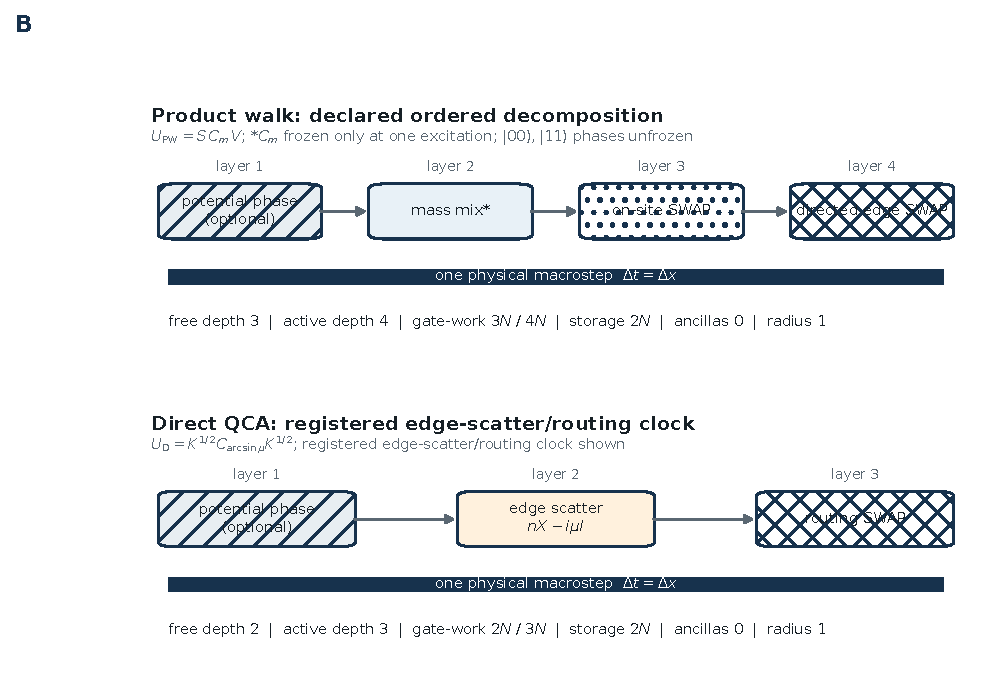
\includegraphics[width=\linewidth]{quantum_dirac_paper/figures/generated/fig02_architecture_comparison.pdf}
  \caption{\textbf{Two registered local circuits under their declared clocks
  (\analytic).}  The product walk uses a mass mixer followed by two SWAP
  transport layers.  The direct QCA uses a mass-bearing edge scatter followed
  by on-site routing.  An active scalar potential contributes one leading
  phase layer.  Counts are exact for the frozen decompositions but are
  nonminimal and change under gate fusion; they are not a hardware compilation
  or an efficiency comparison.  At one excitation the direct block is
  exactly conjugate to a mass-remapped product block by the half-cell
  time-frame change in Eq.~\eqref{eq:time-frame-relation}; the distinction shown
  here is the as-registered decomposition and clock.}
  \label{fig:architectures}
\end{figure}

\begin{table}[t]
  \centering
  \caption{Declared circuit and resource comparison.  Depth and gate-work are
  frozen protocol-clock counts, not optimized compilation minima.}
  \label{tab:architecture-comparison}
  \small
  % Generated table.
\begin{tabular}{@{}p{0.28\linewidth}p{0.32\linewidth}p{0.32\linewidth}@{}}
\toprule
Coordinate & Product walk & Direct symmetry QCA \\
\midrule
Free update & Ordered mass mix and transport & Single normalized QCA block \\
Declared localization & Mass mix; on-site and edge SWAPs & Edge scatter; on-site routing SWAP \\
Full-space scope & Mixer collision phase not frozen & Explicit hard-core $+1$ collision phase \\
Declared free / active depth & $3$ / $4$ layers & $2$ / $3$ layers \\
Declared free / active gate-work & $3N$ / $4N$ & $2N$ / $3N$ \\
Storage; ancillas & $2N$ mode labels; $0$ & $2N$ qubits; $0$ \\
Causal radius & one cell per macrostep & one cell per macrostep \\
Leading free correction & first-order global, Lie--Trotter & second-order global, symmetric time frame \\
Registered refinements & $N=256,512,1024$ & $N=320,640,1280$ \\
\bottomrule
\end{tabular}

\end{table}
